\documentclass[a4paper,12pt,oneside]{report}

\usepackage{fancyhdr}
\usepackage[magyar]{babel}
\usepackage{t1enc}
\usepackage[utf8]{inputenc}
\usepackage{graphicx}
\usepackage{todonotes}
\usepackage[section,numbib,nottoc]{tocbibind}
\usepackage{formai_kovetelmenyek}

\lstset{
     basicstyle = \ttfamily
    ,breaklines = true
    ,prebreak   = \raisebox{0ex}[0ex][0ex]{\ensuremath{\hookleftarrow}}
    ,extendedchars = true
    ,literate={á}{{\'a}}1 {ó}{{\'o}}1 {é}{{\'e}}1 {í}{{\'i}}1
}

\title{Ülésszervezést és jegyzőkönyv-írást támogató keretrendszer készítése}
\author{Fási Gábor}
\date{}

%fattyú- és árvasorok büntetése, ha nagyobb, akkor jobban próbálja elkerülni
\widowpenalty=300
\clubpenalty=300

\graphicspath{{./kepek/}}

\setcounter{secnumdepth}{3} %szamozza a subsubsection-oket is
\AtBeginDocument{\addtocontents{toc}{\protect\pagestyle{empty}}} %ezzel erem el, hogy a tartalomjegyzek ne kapjon oldalszamot
\AtBeginDocument{\addtocontents{tod}{\protect\thispagestyle{empty}}}

\begin{document}
\setcounter{chapter}{1}

\pagestyle{empty}
%------------------------------------------------------------------
% külsõ kötéstábla
{
    \begin{center}
    \vspace*{5cm}
    {
        \Huge SZAKDOLGOZAT}\\
        \vspace*{10cm}
        {\LARGE Fási Gábor}\\
        \vspace*{3cm}
        {\LARGE 2013}
    \end{center}
}
\newpage

% címoldal
\begin{center}
{
    \Large Pannon Egyetem\\
    Villamosmérnöki és Információs Rendszerek
Tanszék\vspace*{3mm}\\
    Mérnök informatikus BSc szak
}
    \vspace*{2cm}\\
    {\LARGE \bf SZAKDOLGOZAT}
    \vspace{3cm}\\
    {\LARGE\bf Ülésszervezést és jegyzőkönyv-írást támogató keretrendszer   készítése}
    \vspace{3cm}\\
    {\large Fási Gábor}
    \vspace{6cm}
    \\
    {\large Témavezető: Dulai Tibor}
    \vspace{1cm}\\
    {\large 2013}
\end{center}
\normalsize
% címlap vége
\newpage

Ide jön az eredeti vagy a fénymásolt feladatkiírás.
\newpage

\begin{center}
\section*{Nyilatkozat}
\end{center}

Alulírott Fási Gábor diplomázó hallgató, kijelentem, hogy a szakdolgozatot a Pannon Egyetem Villamosmérnöki és Információs Rendszerek tanszékén készítettem Mérnök informatikus BSc szak (BSc in Computer Engineering
) megszerzése érdekében.

Kijelentem, hogy a szakdolgozatban lévő érdemi rész saját munkám eredménye, az érdemi részen kívül csak a hivatkozott forrásokat (szakirodalom, eszközök, stb.) használtam fel.

Tudomásul veszem, hogy a szakdolgozatban foglalt eredményeket a Pannon Egyetem, valamint a feladatot kiíró szervezeti egység saját céljaira szabadon felhasználhatja.\\

\begin{flushleft}
{Veszprém, 2013. május 02.\\}
\end{flushleft}

\begin{flushright}
{Aláírás \vspace{4cm}}
\end{flushright}

Alulírott Dulai Tibor témavezető kijelentem, hogy a szakdolgozatot Fási Gábor a Pannon Egyetem Villamosmérnöki és Információs Rendszerek tanszékén készítette Mérnök informatikus BSc szak (BSc in Computer Engineering) megszerzése érdekében.

Kijelentem, hogy a szakdolgozat védésre bocsátását engedélyezem.\\

\begin{flushleft}
{Veszprém, 2013. május 02.\\}
\end{flushleft}

\begin{flushright}
{Aláírás}
\end{flushright}
%A tartalomjegyzék:
\newpage
\pagebreak
\begin{center}
\section*{Köszönetnyilvánítás}
\end{center}
\todo[inline]{Köszönetnyilvánítás}
\newpage

\begin{center}
\section*{\textbf{\Large \MakeUppercase{Tartalmi összefoglaló}}}
\end{center}

\todo[inline]{Tartalmi összefoglaló}

\vspace{2cm}

{\bf Kulcsszavak:} {\it robotfoci, mobil robotika, mikrovezérlõ
programozás, vezeték nélküli kommunikáció, motorvezérlés, hálózati
programozás, Qt, OpenCV }
\newpage

\newpage

\begin{center}
\section*{\textbf{\Large \MakeUppercase{Abstract}}}
\end{center}

\todo[inline]{Abstract}

\vspace{2cm}

{\bf Key words:} {\it robot soccer, mobil robotics, microcontroller programming,
wireless communication, motor control, network programming, Qt, OpenCV }
\newpage
%--------------%------------------------------------------------------------------
\pagenumbering{gobble} %ne legyen oldalszamozas
\listoftodos

\renewcommand{\thefigure}{\arabic{figure}}

\setcounter{tocdepth}{3} %subsubsection-ok is latszodjanak
\thispagestyle{empty}
\thispagestyle{empty}
\tableofcontents
\pagebreak

\pagenumbering{arabic} %legyen oldalszamozas
\setcounter{page}{1} %innentől indul az oldalszámozás
\pagestyle{plain}

\section{A feladat összefoglalása}

Témám egy olyan rendszer elkészítése, mely böngészőn keresztül használható, a megfelelő jogosultságú felhasználók képesek ülést hirdetni helyszínnel, időponttal, majd erre résztvevőket meghívni, akik erről automatikus értesítést kapnak. Szintén a rendszer feladata a lefolyt ülések jegyzőkönyvei elkészítésének segítése, ezek megőrzése és megfelelő feltételek esetén nyilvánossá tétele.

A rendszer fő haszonélvezője a Pannon Egyetem Hallgatói Önkormányzata lesz, de célom a lehetőség általánosítás, hogy a későbbiekben bárki könnyen és gyorsan az egyedi igényeihez tudja szabni és használatba venni.

\section{Hasonló célú hazai és külföldi rendszerek}

Számos jegyzőkönyvvezető rendszer érhető el már magyar nyelven is, de ezek többsége másfélére specializálódott, mint az én rendszerem; például mérési-, verseny vagy vizsgajegyzőkönyv-készítésre.

Három darab ülésjegyzőkönyv-készítő funkcionalitással bíró rendszert találtam, melyek magyar készítésűek:

\begin{itemize}

    \item \emph{AC-TMTR, avagy az Albacomp Testületi Munkát Támogató Rendszer}\cite{website:actmtr}\\
    Önkormányzatok számára készült, honlapjuk szerint ,,Az AC-TMTR a teljes demokratikus döntéshozatali folyamat támogatására alkalmas az előterjesztések kezelésétől a döntések végrehajtásáig''.\\
    A rendszer tudása messze több, mint jegyzőkönyvkészítés, Lotus Notes alapon működik.
    
    \item \emph{InterMap e-FORTE}\cite{website:eforte}\\
    Fő célcsoportja a polgármesteri hivatalok, felső államigazgatás és nagyvállalatok vezetése, ennek tudása is jelentősen meghaladja a jegyzőkönyvkészítést és ülésszervezést.\\
    Webalapú, ASP.NET nyelven készült.
    
    \item \emph{eKÖZIG döntéstámogató rendszer}\cite{website:ekozig}\\
    Szintén a közigazgatás a fő célcsoport, nagyméretű és bonyolult rendszert eredményezve.\\
    Webalapú, ASP nyelven íródott.
    
\end{itemize}

A fenti rendszerek mindegyike fizetős, valamint a mögöttes technológia is \textendash{} az operációs rendszer (Windows) és a futtatókörnyezet (ASP, ASP.NET) egyaránt komoly beruházást igényel a bevezetéskor.

\todo[inline]{Külföldi rendszerek?}

\section{A rendszer tervezése}

A következőkben vázolom a rendszerem felépítését, az egyes komponensek feladatait, azok tervezésével kapcsolatos főbb megszorításokat, döntéseket.

\subsection{Modulok}

A rendszer három fő modulra bontható:

\begin{enumerate}
    \item Felhasználókezelés, authentikáció és authorizáció
    \item Ülések hirdetése, kezelése
    \item Jegyzőkönyvírás
\end{enumerate}

\subsubsection{Felhasználókezelés, authentikáció és authorizáció}

Az alkalmazás zárt, azaz nincs szabad regisztráció, csak az adminisztrátorok hozhatnak létre új felhasználót, illetve ők tudják a létezőket módosítani. A rendszer a kényelmes, gyors és biztonságos bejelentkezésre a Google OpenID rendszerét használja, így nem kell például jelszavak biztonságos tárolásáról gondoskodnunk. Minden HÖK tag rendelkezik egy Google Apps fiókkal.

Ennek a modulnak a feladata az OpenID bejelentkezési folyamat megvalósítása, a kapott adatok alapján a felhasználóhoz párosított jogosultsági szint ellenőrzése a rendszer használata során. Szintén ide tartozik a felhasználók adminisztrátorok általi kezelése.

A felhasználók authentikációjára és authorizációjára a Symfony2 Security komponensét használom \textendash{} ennek segítségével egyéb bejelentkezési módok utólag is kevés munkával hozzáadhatók a rendszerhez. Itt külön említést érdemel a klasszikus, felhasználónévvel (e-mail címmel) és jelszóval történő bejelentkezés, mely néhány sor konfigurációval és egy loginformot tartalmazó template-tel megoldható. Ilyen további bejelentkezési lehetőségek hozzáadásával megoldható, hogy valaki Google fiók nélkül is hozzáférjen a rendszerhez.

\subsubsection{Ülések hirdetése, kezelése}

Az ülések rendelkeznek fix számú adattal, mint a rövid leírásuk, időpontjuk és a helyszínük. Megfelelő jogosultsággal rendelkező felhasználók képesek a fenti adatok megadása után ülést hirdetni, meghívottakat megadni. Opcionális adat még az ülés hosszú leírása, itt lehet például megadni a tervezett napirendi pontokat; valamint lehetőség van dokumentumok feltöltésére, ha valami anyagot előzetesen tanulmányozni kell a résztvevőknek.

A rendszer a hirdetett üléseknek létrehoz egy bejegyzést a Google Naptár alkalmazásában, melyre meghívja a résztvevőket, így az bekerül az ő naptárukba is, valamint erről értesítő levelet kapnak.

\subsubsection{Jegyzőkönyvírás}

A lezajlott ülésekhez készíthető jegyzőkönyv, de természetesen ülés nélkül is lehet jegyzőkönyvet létrehozni (korábbi ülések, vagy ha a szervezés valamely oknál fogva a rendszeren kívül történt).

A jegyzőkönyvek rendelkeznek ugyanazokkal az alapadatokkal, mint az ülések, valamint tetszőleges számú bejegyzéssel, melyekből három típust különböztetünk meg: napirendi pont, felszólalás valamint szavazás. Mind más adatokkal rendelkezik, a rendszernek kezelnie kell ezt, valamint a bejegyzések egymás közti sorrendjét.

A papír alapú iktatást elősegítendő lehetőség van az elkészült jegyzőkönyvek pdf formátumú exportálására.

Szintén e modul feladata a nyilvános ülések kész jegyzőkönyveinek publikálása, bárki számára elérhetővé tétele.

\subsection{Választott technológia}

Feladatom tervezése során hangsúlyt fektettem arra, hogy nyílt forráskódú, ingyenes rendszerekre építsem a megoldásom. A hardverköltségtől eltekintve, amely mindenképpen jelen van, az ilyen szerverek összeállítása a lehető legolcsóbb, illetve szakemberek is bőven állnak rendelkezésre. Így esett választásom a PHP nyelvre és a Symfony2 keretrendszerre.

A választott követelményeimnek megfelelő webszerverekből az egyetem már most is rendelkezik több darabbal, és persze hozzájuk értő rendszergazdákkal is, így a rendszer majdani bevezetésének a költsége minimális.

\subsubsection{PHP}

A php ma az egyik legelterjedtebb programozási nyelv, melyet weboldalak készítésére használnak. Rengeteg kezdőknek szóló leírás van róla, minden webfejlesztő ismeri legalább az alapjait. Bőségesen áll rendelkezésre akár ingyenes tárhely is, ahová felrakhatjuk az elkészült programunkat.

A 2008-ban megjelent 5.3-as verzióval a nyelvbe bekerült a névterek támogatása, valamint a garbage collector algoritmusa is sokat javult, jelentős teljesítmény\-növe\-kedést eredményezve. A feladatom minimum követelménye az 5.3.7-es verzió, ebben javítottak egy, a bcrypt modulban levő hibát, mely hibás (viszonylag könnyen törhető) jelszókódolást eredményezett.

\subsubsection{Symfony2}

A Symfony az egyik nagy keretrendszer a php világában. Első verziója 2005-ben jelent meg\cite{book:gentle_introduction}, csak ragasztó volt egy maréknyi könyvtár közt, azok együttes használatát segítendő. Folyamatosan fejlődött, olyan nagy oldalak hasz\-nálták, mint a Yahoo!\cite{website:symfony_yahoo} és a Dailymotion\cite{website:symfony_dailymotion}. Az 1.4-es ága 2009-ben jelent meg, és egészen 2012 novemberéig rendelkezett támogatással.

A Symfony2 hosszas fejlesztést követően jelent meg 2011 júliusában. Az egyik első nagy keretrendszer volt, mely a php5.3 új lehetőségeit kihasználva lett az alapoktól újraírva. Fejlődése a közösség bevonásával történt, több, mint 250 önkéntes segített be. Mostanra 600 feletti a fejlesztésben részt vevők száma.

A rendszerem fejlesztése a 2.1-es verzióban történt. A készítés utolsó hónapjaiban adták ki a 2.2-es verziót számos visszafelé nem kompatibilis változtatással, ezért nem frissítettem rá \textendash{} a 2.1-es változat 2013 közepéig élvez hivatalos támogatást, így a rendszer további fejlesztése során mindenképpen megfontolandó a 2.2-re átállás.

A Symfony remekül együtt tud működni a Doctrine ORM-el\cite{website:doctrine,book:doctrine_orm}, ezzel lehetővé téve, hogy az alkalmazásunk számára észrevétlenül lecseréljük az adatbázis-szerverünk valamely más típusúra. A tábláink szerkezetét egy egységes módon kell megadnunk, és az illesztőfüggő kódot a Doctrine legenerálja nekünk. Szintén jó a támogatása az adatbázis-migrációkkal kapcsolatban, ha változik az adataink szerkezete, ezt nem kézzel kell lekövetnünk az éles szerveren, egyetlen, a terminálban kiadott paranccsal a Doctrine ezt megteszi nekünk.

\subsubsection{Bootstrap}

A Twitter által megalkotott Bootstrap\cite{website:bootstrap} css keretrendszer segítségével könnyen és gyorsan hozhatunk létre egységes, jól kinéző webalkalmazásokat. Beépítve tartalmaz egyszerű, de jól használható stílusokat a webfejlesztés szinte minden területére, az alapkinézet megalkotásától az űrlapmezők formázásáig. Élénk közösség alakult ki körülötte, így a korábban nem lefedett területekre is számos megoldás létezik mostanra. A kezdetek óta kiegészült egy maréknyi javascript könyvtárral is, melyekkel egyszerűen tudunk például dialógusablakokat vagy hasonló, gyakori feladatokat megoldani.

\subsection{Kritikus részek}

A következőkben megemlítem a rendszer kritikus pontjait, illetve hogy milyen tervvel rendelkezem ezek megoldására.

\subsubsection{OpenID authentikáció}

Az OpenID\cite{website:openid_specifikacio} egy viszonylag összetett protokoll sok hibázási lehetőséggel. Szerencsére több készen elérhető megoldás is létezik, ezek közül nem egy pedig minimális konfiguráció után kész együttműködni a Symfony2 biztonsági komponensével köszönhetően annak, hogy készítettek hozzá kiterjesztést (a Symfony terminológiában Bundle-t). Ezek közül az FpOpenIdBundle\cite{website:fpopenidbundle}-t választottam.

\subsubsection{Jogosultságkezelés}

A jogosultságok kiosztásában olyan rugalmasnak kell lennünk, amit egy egyszerű, felhasználókat csoportokra bontó megoldás nem tesz lehetővé. Az egyeztetések során hamar kiderült, hogy több olyan felhasználó is lesz, aki az eredeti rendszer szerint nem hirdethetne ülést (mert nem kari elnök), de ezt mégis lehetővé kell tenni számára.

A Symfony2 Security komponense nagyon finom jogosultság-szabályoztást tesz lehetővé onnantól, hogy egy oldalt valaki csak megfelelő joggal ér el, odáig, hogy egy adott adatbázis-rekord valamely mezőjéhez hozzáférhet-e.

\subsubsection{Google Naptár együttműködés}

Az API, amivel eseményeket lehet létrehozni és arra meghívottakat hozzáadni\cite{website:gcal_event_api} nincs túlbonyolítva, és a Google ad php-hoz hivatalos klienskönyvtárat\cite{website:google_api_client}. Ennek segítségével hoztam létre egy Symfony2 szolgáltatást, mellyel a rendszer bármely részéről könnyen tudok a Naptárral kapcsolatba lépni.

A rendszer a meghirdetett ülésekről létrehoz egy-egy naptárbejegyzést, és az ülés meghívottjait ott is felveszi a meghívottak közé \textendash{} így ez bekerül az ő naptárukba is.

\subsubsection{PDF exportálás}

Webes rendszerek esetén gyakran előforduló kérés, hogy valamely generált dokumentumot lehessen pdf-ben is letölteni; így nem meglepő, hogy számos Symfony2 Bundle foglalkozik ezzel a feladattal.

Választásom egy olyan könyvtárra esett, mely HTML bemenet alapján generálja a PDF kimenetet, így a későbbiekben a nyomtatott jegyzőkönyv kinézete, az elemek sorrendje, formátuma könnyen módosítható a felhasználók igényei szerint.

\subsection{Felületterv}

Az következőkben bemutatom a rendszer három várhatóan leggyakrabban látogatott képernyőjét. Az elrendezése mindegyiknek ugyanaz: felül egy menüsáv, ahol a bejelentkezett felhasználó jogosultsági szintjétől függően látszanak a menüpontok.

\subsubsection{Kezdőlap}

Bejelentkezés után minden felhasználó erre az oldalra érkezik. Áttekintő táblázatot kap az elkövetkező üléseiről, illetve azon jegyzőkönyveiről, melyek már létre lettek hozva, de még nincsenek lezárva. Ennek terve látható a \ref{fig:wireframe-kezdolap}. ábrán.

\begin{figure}[h]
    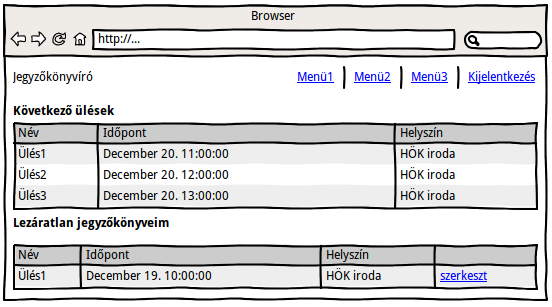
\includegraphics[width=\textwidth]{wireframe-kezdolap}
    \caption{A bejelentkezettek kezdőlapjának látványterve}
    \label{fig:wireframe-kezdolap}
\end{figure}

\subsubsection{Üléshirdetés}

Ezen a képernyőn lehet megadni az ülés alapadatait és résztvevőket meghívni. Ennek terve látható a \ref{fig:wireframe-uleshirdetes}. ábrán.

\begin{figure}[h]
    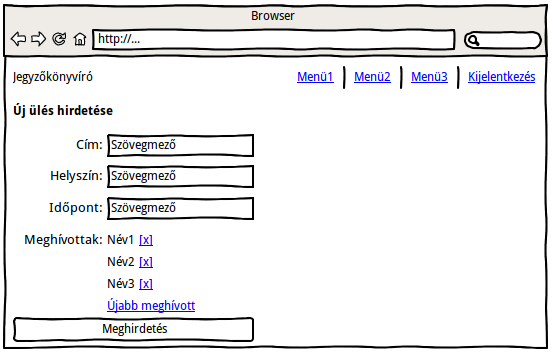
\includegraphics[width=\textwidth]{wireframe-uleshirdetes}
    \caption{Az ülés hirdetésére szolgáló űrlap látványterve}
    \label{fig:wireframe-uleshirdetes}
\end{figure}

\subsubsection{Jegyzőkönyvírás}

Itt tudja az írással megbízott felhasználó felvinni a jegyzőkönyv elemeit, melyek sorrendfüggően egymás alatt látszanak. Ennek látványterve található a \ref{fig:wireframe-jegyzokonyvszerkesztes}. ábrán.

\begin{figure}[h]
    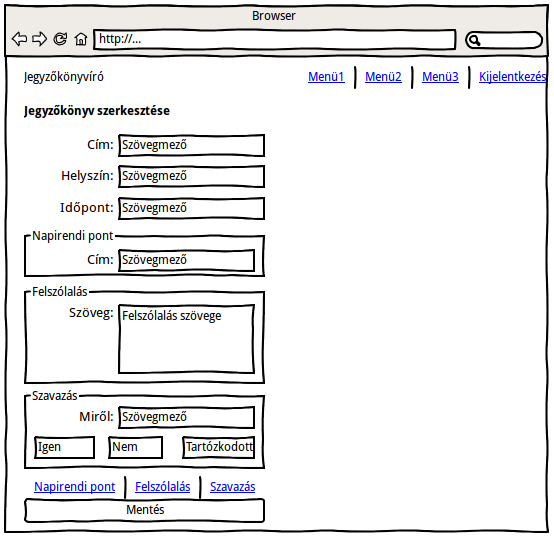
\includegraphics[width=\textwidth]{wireframe-jegyzokonyvszerkesztes}
    \caption{A jegyzőkönyv szerkesztésére szolgáló felület látványterve}
    \label{fig:wireframe-jegyzokonyvszerkesztes}
\end{figure}

\subsection{Jogosultságok leírása}

Néhány mondatban szót ejtek a rendszer által kezelt jogosultságokról, illetve hogy kik lesznek a jellemző tulajdonosai.

%csillagozva nem kap számozást, és a tartalomjegyzékbe sem kerül be
\subsubsection*{Felhasználó}

Az alapszintű jogosultság, hozzáfér a rendszerhez, képes jegyzőkönyveket létrehozni (üléshez párosítva is, illetve önmagában, a rendszeren kívül szervezett ülésekről) és megírni, illetve azon ülések részleteihez és feltöltött anyagaihoz hozzáférni, ahol meghívottként szerepel.

Nem kell külön kiosztani, megkapja mindenki, aki a rendszerhez hozzáféréssel rendelkezik.

\subsubsection*{Üléshirdető}

A fentieken kívül tud még ülést hirdetni, annak jegyzőkönyvírásával megbízni valakit, illetve természetesen az üléseinek adatait szerkeszteni, azokhoz dokumentumokat feltölteni.

Jellemzően a kari HÖK elnökök kapják majd ezt a jogot, de rajtuk kívül más személyek is, akik valamely vezető tisztségben vannak.

\subsubsection*{Adminisztrátor}

A fentieken kívül képes a felhasználók kezelésére, adataik megadására (teljes név, szervezeti egység azon belüli pozíció), illetve jogosultságaik kiosztására. Képes tetszőleges ülés adatait és meghívottait módosítani.

Kezdetben egyetlen ilyen jogú felhasználó lesz, a későbbiekben ez az egy igény szerint tud létrehozni újabbakat.

\subsection{Jegyzőkönyv létrehozásának folyamata}

Egy jegyzőkönyv létrehozása az ülés hirdetésétől kezdve a következő lépésekből áll:

\begin{enumerate}
  \item \emph{Ülés hirdetése}\\
    Egy arra jogosult személy meghirdet egy ülést, megadja annak alapadatait (név, helyszín, napirendi pontok), meghívja a résztvevőket.
    
  \item \emph{Ülés jegyzőkönyvírójának megadása}\\
    Az ülés hirdetője a meghívottak közül kiválasztja a jegyzőkönyvírással megbízott személyt, valamint a jegyzőkönyv két hitelesítőjét.
    
  \item \emph{Jegyzőkönyv alapadatainak megadása}\\
    A jegyzőkönyv írója kiválaszthatja, hogy melyik ülés jegyzőkönyvét írja, ekkor a rendszer az ismert adatokat átemeli onnan. Alternatívaként létrehozhat jegyzőkönyvet üléshez párosítás nélkül is, azon eseteket kezelendő, mikor az ülés szervezése a rendszeren kívül történt.

  \item \emph{Jegyzőköny megírása}\\
    A megbízott megírja a jegyzőkönyvet tetszőleges számú bejegyzést hozva létre.
    
  \item \emph{Jegyzőkönyv lezárása}\\
    A jegyzőkönyv írója a folyamat végén lezárja a jegyzőkönyvet, innentől ez nem módosítható.

  \item \emph{Jegyzőkönyv hitelesítése}\\
    A jegyzőkönyv két kijelölt hitelesítője a kezdőlapjukon a megfelelő táblázatban látják, hogy elkészült a jegyzőkönyv. Ezt meg tudják tekinteni, és ha mindent rendben találnak, egy gombnyomással hitelesnek jelölhetik.

    Ha valamelyik hitelesítő hibát talál, erről értesítést tud küldeni a jegyzőkönyv írójának. Ekkor a jegyzőkönyv lezárása is feloldódik, hogy az ismét szerkeszteni tudja.

  \item \emph{Jegyzőkönyv elkészülte}\\
    Mikor mindkét hitelesítő jelezte, hogy a jegyzőkönyv helyes, erről az Ellenőrző Bizottság a beállított e-mail címre értesítést kap, továbbá ha az jegyzőkönyv nyilvános, az publikálásra kerül a rendszer egy bárki számára elérhető oldalán.

\end{enumerate}

Ha a jegyzőkönyv elkészülte után bármilyen okból szükség van erre, a jegyzőkönyvet egy adminisztrátor vissza tudja helyezni szerkeszthető állapotba. Ekkor az írója ismét módosíthat rajta, és a teljes lezárási-hitelesítési folyamatot meg kell ismételni.

A folyamat úgy van kitalálva, hogy két felhasználóra oszlanak a fő feladatok: az ülés hirdetőjére és a jegyzőkönyv írójára. Természetesen a két személy lehet ugyanaz, ha az ülés hirdetője a jegyzőkönyvíró szerepét önmagának osztja ki.

\subsection{Tesztelési terv}

A Symfony2 remekül támogatatja az egység- és funkcionális tesztek írását. Ezt lehetőségeimhez mérten igyekszem kihasználni megelőzve azt, hogy a fejlesztés későbbi részeiben valami már működő funkcionalitást elrontsak.

\todo[inline]{Tesztelésről részletesebben}
Szintén hasznát fogom venni a Travis-CI szolgáltatásnak, melynek lényege az, hogy minden verziókövetőbe történő commit után automatikusan lefuttatja a teszteket akár több PHP verzión, illetve adatbázis-szerveren.

Emellett amint a rendszer eléri a megfelelő fejlettségi szintet, telepítésre kerül egy alkalmas szerverre, hogy valós felhasználók is elkezdhessék annak próbálgatását és visszajelzések küldését.

\section{Fejlesztési napló}

A rendszer moduljainak fejlesztési sorrendje azok egymásra épülései miatt a következő volt:

\begin{enumerate}
  \item \emph{Felhasználók}\\
    Ebben a szakaszban készült el a bejelentkezési folyamat, a felhasználóhoz jogainak hozzárendelése, valamint a felhasználók kezelésére szolgáló rész: azok listázása, új felvétele, létezők szerkesztése.
    
  \item \emph{Ülések}\\
    Elkészült az üléshirdetési folyamat meghívással, egyelőre a Google Calendar integráció nélkül. Működik a dokumentumfeltöltés, valamint az ülések listázása több szempontból, mint például a saját üléseim, vagy azok, amelyekre meghívtak.
    
  \item \emph{Jegyzőkönyvek}\\
    Megvalósításra került a jegyzőkönyvek készítésére szolgáló modul. Lehet újat létrehozni csak úgy, illetve üléshez kapcsolva is. A pdf exportálás későbbre marad.\\
    Ez a szakasz volt a legidőigényesebb.
    
  \item \emph{Tesztelés}\\
    A rendszer alapvető funkciói elkészültek, így az telepíthető volt egy arra alkalmas szerverre, hogy elkezdődhessen az éles üzemre való felkészítés, illetve hogy valós felhasználói vélemények alapján tudjam a működést finomhangolni.
    
  \item \emph{Naptáresemény és exportálás}\\
    Megvalósult a Google Naptárral kommunikáló szolgáltatás, hogy a hirdetett ülésekről ott is létrejöjjön esemény, valamint a kész jegyzőkönyvek PDF formátumban történő exportálási lehetősége.
\end{enumerate}

\section{A fejlesztés részletei}

A következőkben modulokra bontva részletezem a fejlesztés menetét, a főbb lépéseket, a tapasztalt kihívásokat. Előbb azonban ismertetnék néhány fontos koncepciót a Symfony2 felépítéséről és működéséről.

\subsection*{A Bundle rendszer}

A symfony 1-es verziója egy monolitikus rendszer volt, nem lehetett egyes komponenseket könnyen cserélni alternatív megoldásokra. Támogatta pluginek használatát, de központi rendszereket ezek sem tudtak helyettesíteni, illetve a nem általános használati esetekben nagyon körülményesek voltak.

A korábbi tapasztalatokra építve a Symfony2-ben új megoldást használtak, ez lett a bundle rendszer\cite{website:symfony2_bundle}. Ez hasonló a pluginekhez, a fontos különbség az, hogy a keretrendszerben \emph{minden} bundle, annak központi funkciói is \textendash{} ezzel elérték azt, hogy moduláris, könnyen bővíthető rendszert adjanak ki.

Az alkalmazásunk valójában egy minimális, főleg konfigurációból álló ragasztó az azt felépítő bundle-ök körül; ezeket pedig az alkalmazásunk \texttt{AppKernel.php} file-jában regisztráljuk:

\begin{lstlisting}
class AppKernel extends Kernel
{
    public function registerBundles()
    {
        $bundles = array(
            // fentebb kihagyva a keretrendszer alapjai,
            // utana a sajatjaink
            new SzakdolgozatSzakdolgozatBundle(),
            new SzakdolgozatFelhasznaloBundle(),
            new SzakdolgozatUlesBundle(),
            new SzakdolgozatJegyzokonyvBundle(),
        );

        return $bundles;
    }
}
\end{lstlisting}

Ezeket persze lehet feltételesen regisztrálni, azaz megtehetjük, hogy egy adott (mondjuk automatikus naplózáshoz használt) bundle csak az éles szerveren van használva, tesztkörnyezetben nem.

Egy bundle egy adott funkcióhoz szükséges összes file gyűjteménye. Ez lehet néhány alapfunkció is, mint mondjuk néhány adatbázis-tábla leírása és a hozzájuk tartozó osztályok, a másik véglet mondjuk egy egész fórumrendszer. Van néhány általános ajánlás a felosztásra. Semmi nincs kőbe vésve, minden a fejlesztő döntésein múlik.

\subsection*{A Dependency Injection Container}

Erre a komponensre nyugodt szívvel lehet mondani, hogy a keretrendszer lelke, az, ami összefogja az egészet. Viszonylag kisméretű (kb. 10k LOC), de óriási lehetőségek rejlenek benne.

Ennek a komponensnek segítségével egy helyen tudjuk leírni, milyen szolgáltatásai vannak a bundle-ünknek, azokat milyen azonosítóval lehet elérni, illetve milyen paraméterek szükségesek a példányosításához, helyes működéséhez. Támogatottak a kötelező függőségek (konstruktoros paraméterátadás) és az opcionálisak is (setteres átadás). A definiált szolgáltatások egésze, vagy akár csak egy-egy paramétere módosítható az alkalmazás szintjén, vagy egy, a mienkre épülő bundle-ben. Paraméterként használhatóak skaláris értékek, de akár egy másik szolgáltatás is.

A szolgáltatások leírása szövegesen, yaml vagy xml formában történhet. Ezek értelmezése lassú folyamat, ami nem megengedhető éles környezetben. Ezen segítendő ezek csak a gyorsítótár ürítése utáni első kéréskor vannak parse-olva, a későbbiek egy php-re fordított és mentett, tehát nagyon gyors változatot használnak.

Példaként álljon itt egy szolgáltatás a \texttt{SzakdolgozatFelhasznaloBundle}-ből:

\begin{lstlisting}[]
szakdolgozat.felhasznalo.felhasznalo_param_converter:
    class: Szakdolgozat\FelhasznaloBundle\Request\ParamConverter\FelhasznaloParamConverter
    arguments: [@doctrine.orm.default_entity_manager]
    tags:
        - { name: "request.param_converter" }
\end{lstlisting}

Ebben a példában egy úgynevezett ParamConverter szolgáltatást írok le, ezekről a felhasználó modul leírásakor részletesebben lesz szó. Ennek egy konstruktorban átadandó paramétere van, ami egy másik szolgáltatás, a doctrine entity managere. Végül adok neki egy adott névvel rendelkező cimkét \textendash{} amikor a container összeállításra kerül, ezek alapján is lekérdezhetőek a service-ek, és megfelelően használhatóak.

\subsection*{Konfigurációs lehetőségek}

Ahogy majdnem mindenre, konfigurációra is több alternatívánk van. Természetesen létezik ajánlás is, amit érdemes követni, ha a bundle-ünket szeretnénk később publikálni.

Az első lehetőség az XML file-ok használata. Nagy előnye, hogy széleskörűen ismert és jóldefiniált formátum, félreértési lehetőségek nélkül. A symfony.com alatt találhatóak hozzá XSD sémák, ezek segítségével a megfelelő szerkesztőkben kódkiegészítést is kapunk. Hátránya, hogy nagyon bőbeszédű.

A második lehetőség a YAML formátum. Ez szintén egyszerű szöveges formátum, a hierarchia jelölésére szóközökkel való behúzást használ. Például a nem sokkal fentebbi, ParamConverter szolgáltatást regisztráló kódrészlet yaml formátumban van. Előnye, hogy kevés benne a felesleges szöveg, azaz szemmel is könnyen és gyorsan értelmezhető. Hátránya, hogy időnként nem egyértelmű, és a parser hibaüzenetei is gyakran nagyon megtévesztőek.

A harmadik lehetőség az annotációk használata. Más nyelvekben, például java-ban ez már régóta nyelvi szinten támogatott, php-ban ilyen nincs, segédkönyvtárak alkalmazása szükséges. A Symfonyban a Doctrine Common ezen része használatos, ez a \lstinline!/**!-al kezdődő kommenteket értelmezi DocBlock-ként. Előnye, hogy a kód és a konfigurációja egy helyen van, hátránya, hogy a nyelv szempontjából kommentben elrejtve, ami egyeseket zavarhat, illetve bizonyos opcode cache-ek ezeket kioptimalizálják, nem működő kódot eredményezve.

Kutatásom alapján az adatbázis-entitások leírására leginkább használt formátum az annotáció, minden másra a yaml, így a szakdolgozatom fejlesztése során is ezeket használtam.

\subsection{Felhasználó modul}

Az összes többi modul épít a felhasználókra, így ezt volt logikus elsőnek elkészíteni. A következőkben részletezem a belső felépítését és működését.

\subsubsection*{Adatbázisának szerkezete}

A hozzá tartozó táblák tartalmazzák a felhasználókat, a rendszer által ismert jogokat, illetve hogy ebből melyik felhasználó melyekkel rendelkezik. Ennek szerkezete látható az \ref{fig:felhasznalo_db}. ábrán.

\begin{figure}[h]
  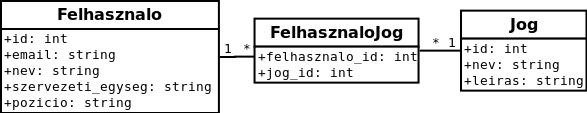
\includegraphics[width=\textwidth]{felhasznalo_db.png}
  \caption{A felhasználó modul adatbázis-szerkezete}
  \label{fig:felhasznalo_db}
\end{figure}

A felhasználók OpenID-n keresztüli azonosítása az email címük alapján történik, így ezen a mezőn egyedi megszorítás van. Az id mezőt automatikusan számozza az adatbázis-szerver, ez a tábla elsődleges kulcsa; a felületen megjelenítve sehol nincs, de másik táblák ez alapján hivatkoznak egy bizonyos felhasználóra.

A jog tábla tartalmazza a rendszer által ismert jogokat. A felületen ezek nem szerkeszthetők, az, hogy ezeket nem beégettem a kódba, hanem adatbázisban tárolom, a további fejlesztést teszi könnyebbé. Minden jog rendelkezik egy névvel és egy leírással, felhasználók létrehozásakor és szerkesztésekor ezeket az adminisztrátorok látják.

Az ide tartozó harmadik tábla segédtába, a felhasználó és a jog tábla közötti több-több kapcsolat teszi szükségessé. Egyéb információt nem is tárol, csak (felhasználó, jog) rendezett párokat. A két mező együtt az elsődleges (és így egyedi) kulcs.

\subsubsection*{Használati esetek}

A rendszer használati esetei közé tartozik a felhasználók azonosítása, ennek a folyamatnak része azok jogainak munkamenetbe mentése is; illetve az azok kezelésével kapcsolatos folyamatok: listázás, létrehozás, szerkesztés és törlés, ezek összefoglaló neve a CRUD\cite{website:crud}.

\begin{figure}[h]
    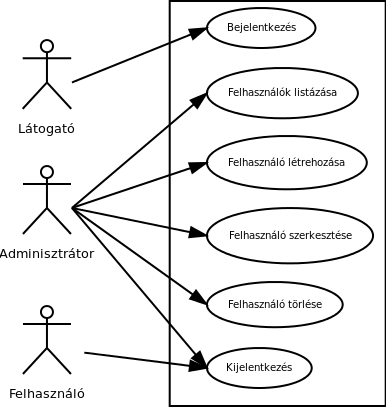
\includegraphics[width=0.8\textwidth]{felhasznalo_usecase.png}
    \caption{A felhasználó modul használati esetei}
    \label{fig:felhasznalo_usecase}
\end{figure}

A modul felhasználói esetei láthatóak a \ref{fig:felhasznalo_usecase}. ábrán.

\subsubsection*{Adatbázis-osztályok}

A megvalósítás első lépése az adatbázis tábláinak létrehozása volt. Mivel a Doctrine-nal dolgozom, ezért ezt úgy csináltam, hogy táblánként létrehoztam egy-egy PHP osztályt, és jeleztem a Doctrine-nak, hogy ezek olyan entitások, amiket tárolni szeretnék. Erre annotációkat használtam. Példaként álljon itt a {\tt Felhasznalo} osztály egy részlete:

\begin{lstlisting}
/**
 * @ORM\Entity(repositoryClass="Szakdolgozat\FelhasznaloBundle\Entity\FelhasznaloRepository")
 * @ORM\Table(name="felhasznalo")
 */
class Felhasznalo implements UserInterface
{
    /**
     * @ORM\Id
     * @ORM\Column(type="integer")
     * @ORM\GeneratedValue(strategy="AUTO")
     */
    protected $id;

    /**
     * @ORM\Column(type="string", length=100, unique=true, nullable=false)
     */
    protected $email;
}
\end{lstlisting}

A példában az {\tt ORM}-mel kezdődő annotációkkal foglalkozik a Doctrine. A megvalósított interfész a Symfony2 Security komponensének jelzi, hogy ez az osztály a rendszer felhasználóit tárolja. Erről később írok bővebben.

Az első kettő, az {\tt Entity} és a {\tt Table} jelzi, hogy itt ez egy tárolandó osztály, az adott nevű táblába, és a megadott repository osztállyal \textendash{} ez az, ahol az egyedi lekéréseinket tudjuk tárolni egy helyen, hogy az könnyen elérhető legyen például a controllerünkből.

Az {\tt id} mezőnél jelezzük, hogy ez azonosító lesz, a mező típusa egész, és hogy az adatbázismotor alapértelmezett generálási sémáját használja \textendash{} MySQL esetén ez az auto\_increment, MSSQL-nél az identity, PgSQL-nél pedig a sequence.

Az email már egyszerűbb, itt csak annyit kell jeleznünk, hogy legfeljebb milyen hosszú karaktersorozatot szándékozunk tárolni, valamint hogy a mező kötelező (azaz nem tartalmazhat null vagy üres értéket), illetve egyedi kell legyen.

Ennek az osztálynak még érdekessége a jogokkal fennálló több-több kapcsolata, ezt az alábbi módon jelzem annotációval:

\begin{lstlisting}
/**
 * @ORM\ManyToMany(targetEntity="Jog", inversedBy="felhasznalok")
 * @ORM\JoinTable(name="felhasznalo_jog")
 */
protected $jogok;
\end{lstlisting}

Azaz egészen egyszerűen csak mondani kell, hogy több-több kapcsolatot szeretnék a {\tt Jog} entity-vel, és a kapcsolótábla neve legyen {\tt felhasznalo\_jog}. Az {\tt inversedBy} mondja meg, hogy a {\tt Jog} entity melyik tulajdonsága ennek a relációnak az ellentéte, abban az osztályban ez a mező így néz ki:

\begin{lstlisting}
/**
 * @ORM\ManyToMany(targetEntity="Felhasznalo", mappedBy="jogok")
 */
protected $felhasznalok;
\end{lstlisting}

Itt a kapcsolótáblát már nem kell megadnunk, fontos viszont, hogy az {\tt inversedBy} helyett {\tt mappedBy} tulajdonságot adunk meg. Ezzel tudjuk jelezni, hogy a kapcsolatnak melyik a tulajdonosi oldala, jelen esetben a felhasználó, azaz hozzá tartoznak a jogok, nem pedig a jogokhoz a felhasználók. Ennek az elemek szerkesztésekor van jelentősége: a Doctrine csak a tulajdonosi oldalt vizsgálja, hogy történt-e változás, kell e módosítani valamely táblát.

\subsubsection*{OpenID}

A protokoll két felet definiál, a {\em providert} és a {\em consumert}. A provider a szolgáltató, ahol a felhasználó rendelkezik már fiókkal, és annak engedélyével megkaphatjuk a kért adatait. A consumer a fogyasztó, jelen esetben a rendszerem, ahová a felhasználó szeretne bejelentkezni a másik oldalnál található fiókjával. A kérés során szabadon megmondhatjuk, hogy a szolgáltatónál elérhető adatok közül melyiket szeretnénk megkapni. Ezek egy része a protokollban van definiálva, de természetesen létre lehet hozni egyedi mezőket is.

A rendszerem tervezésekor még nem tudtam, mennyire összetett ennek a megvalósítása a Symfony keretrendszerben, ezért csak egy szolgáltatóval (Google) történő azonosítást vállaltam. Most már tudom, hogy köszönhetően annak, csak az email mezőre van szükségem, nagyon kevés plusz munkával bármely OpenID kiszolgálóval megvalósítható a bejelentkezés.

A két fél közti kommunikációt a korábban már említett {\tt FpOpenIdBundle} segítségével valósítottam meg.

\subsubsection*{Bejelentkezés}

A rendszer biztonságára az Symfony2 Security komponense ügyel. Előszöris az alkalmazásom {\tt security.yml} fájljában be kellett állítanom, hogy az egész rendszerhez OpenID-n keresztüli bejelentkezés szükséges:

\begin{lstlisting}
access_control:
    - { path: ^/login_openid$, roles: IS_AUTHENTICATED_ANONYMOUSLY }
    - { path: ^/, role: IS_AUTHENTICATED_OPENID }
\end{lstlisting}

A szolgáltatótól kapott adatok ellenőrzését a {\tt /login\_openid} url-en elérhető controller végzi, így azt el kell tudni érni azonosítás nélkül.

A következő lépés az FpOpenIdBundle konfigurálása volt:

\begin{lstlisting}
fp_openid:
    create_user_if_not_exists: true
    provider: openid_user_manager
    required_attributes:
        - contact/email
\end{lstlisting}

A {\tt create\_user\_if\_not\_exists} beállítás neve megtévesztő, ugyanis nem azt jelenti, hogy hozzon létre felhasználót, ha valaki anélkül próbál bejelentkezni. OpenID-ban egy felhasználó több úgynevezett {\em identity}-vel rendelkezik, és a beállítás azt mondja meg, hogy ha új identity-vel érkezik egy felhasználó, azzal beengedje-e. A {\tt provider} egy szolgáltatás nevét tartalmazza, amelynek a feladata a providertől kapott adatokból annak eldöntése, hozzáférhet-e a felhasználó a rendszerhez. Az utolsó érték azt mondja meg, mely adatokat szeretnénk megkapni, jelen esetben ez csak az email cím.

A providerként megadott szolgáltatás egy adott interfészt kell megvalósítson, ami egyetlen függvényt tartalmaz. Bemeneti paramétere a szolgáltatótól kapott adatok tömbje, és a végén vissza kell adnia azt a {\tt Felhasznalo} példányt, akit ezek azonosítanak. Ha nincs az adatok közt email cím, vagy ilyennek rendelkező felhasználónk nincs, akkor a függvénynek exceptiont kell dobnia.

\todo[inline]{szekvenciadiagram?}

Sikeres bejelentkezés után a felhasználó munkamenetébe mentem annak jogait, később ennek függvényében láthat menüpontokat, illetve linkeket. Ezek természetesen szerveroldalon is ellenőrizve vannak, tehát ha egy Adminisztrátor joggal nem rendelkező felhasználó meglátogatja a {\tt /felhasznalo/uj} címet, akkor csak egy hibaoldalt kap.

\subsubsection*{Felhasználók listázása}

A modul funkcióinak fele elkészült, már csak lehetővé kell tennünk, hogy az adminisztrátorok szabadon tudjanak felhasználókat létrehozni, módosítani.

Symfony2-ben a routingot yaml fájlok segítségével tudjuk testreszabni. Külön ilyen létezik alkalmazás- és modulszinten. A moduléban így írtam le a felhasználókat listázó (index) actiont:

\begin{lstlisting}
szakdolgozat_felhasznalo_felhasznalo_index:
    pattern:    /
    defaults:  { _controller: SzakdolgozatFelhasznaloBundle:Felhasznalo:index }
\end{lstlisting}

Az első sor a route neve, a későbbiekben amikor linket generálunk, ezzel tudunk rá hivatkozni úgy, hogy ha a mintát módosítjuk, akkor a linkjeink továbbra is működni fognak. A mintája az adott mappa gyökerére mutat, ezt az egyik következő bekezdésben indoklom. Végül megmondom, hogy ha ez a route illeszkedik a kértre, akkor az aktuális modul {\tt Felhasznalo} controllerének {\tt index} actionjét kell meghívni.

Ettől még nem lesz elérhető ez a route-unk, alkalmazásszintre importálni kell:

\begin{lstlisting}
szakdolgozat_jegyzokonyv:
    resource: "@SzakdolgozatJegyzokonyvBundle/Resources/config/routing.yml"
    prefix:   /jegyzokonyv
\end{lstlisting}

Itt leírom, melyik fájlt kell importálni, valamint hogy milyen előtagot kapjon az abban leírt összes útvonal, így a felhasználók listázása a {\tt /felhasznalo/} linken érhető el. Mivel ezt, és a modul ide tartozó összes linkjét csak adminisztrátorok láthatják, a security konfigban védjük is le rögtön:

\begin{lstlisting}
- { path: ^/felhasznalo, role: ROLE_ADMINISZTRATOR }
\end{lstlisting}

ezt a sort a Bejelentkezés szekcióban mutatott két hozzáférési szabály közé kell írni.

A következő lépés a lista linkelése a menübe. A keretrendszerrel több template nyelv támogatás érkezik beépítve, ebből én a Twiget\cite{website:twig} választottam. Az alapvető vezérlési szerkezetek megtalálhatóak benne, és a Symfony számos függvénnyel kiegészíti, például ezzel, amelyikkel azt tudjuk ellenőrizni, a bejelentkezett felhasználónk jelentkezik-e egy adott joggal:

\begin{lstlisting}

<li><a href="{{ path('szakdolgozat_felhasznalo_felhasznalo_index') }}">Felhasználók</a></li>

\end{lstlisting}

Ezután már elkészíthetjük a controllerünk erre az url-re meghívott függvényét. A konvenció szerint a routingban megadott {\tt index} értékre a Symfony a {\tt indexAction} nevű függvényt keresi. Ez a függvény a következőképp néz ki:

\begin{lstlisting}
public function indexAction()
{
    $felhasznalok = $this->getDoctrine()->getRepository("SzakdolgozatFelhasznaloBundle:Felhasznalo")->findAll();

    return $this->render("SzakdolgozatFelhasznaloBundle:Felhasznalo:index.html.twig", array(
        "felhasznalok" => $felhasznalok,
    ));
}
\end{lstlisting}

Azaz lekérjük az összes felhasználót, majd átadjuk a twig template-ünknek. A {\tt findAll} függvény alapértelmezetten az adatbázisbeli sorrendben adja vissza a rekordokat, nekünk ez nem jó, név szerinti ABC-rendezést szeretnénk. Korábban, a {\tt Felhasznalo} entity leírásánál már láthattuk, hogy ez egy saját {\tt Repository} osztállyal rendelkezik, ahol a {\tt findAll} függvényt így definiálom:

\begin{lstlisting}
public function findAll()
{
    return $this->createQueryBuilder("f")
        ->select("f")
        ->orderBy("f.nev", "ASC")
        ->getQuery()
        ->getResult();
}
\end{lstlisting}

ami az alapértelmezett megvalósítástól egyedül a rendezést leíró sorban tér el.

Utolsó lépésként a megfelelő template fájlban végig kell iterálnunk a kapott felhasználókon, kiírni a megjeleníteni szándékozott adataikat, illetve egy szerkesztés linket:

\begin{lstlisting}

<tr>
    <td>{{ f.nev }}</td>
    <td>{{ f.email }}</td>
    <td>{{ j.nev }}, </td>
    <td><a href="{{ path("szakdolgozat_felhasznalo_felhasznalo_edit", { "id": f.id }) }}">szerkesztés</a></td>
</tr>

\end{lstlisting}

ebben a kódrészletben két példát is láthatunk a {\tt for} ciklusra: a külső a felhasználókon megy végig, a belső pedig azok jogain, végeredménye a jogok vesszővel elválasztott névsora lesz. A kimenete látható a \ref{fig:felhasznalo_lista}. ábrán.

A táblázat utolsó cellája egy olyan link lesz, amelyet meglátogatva az a felhasználó szerkeszthető. A következő szakaszban ezt részletezem.

\begin{figure}[h]
    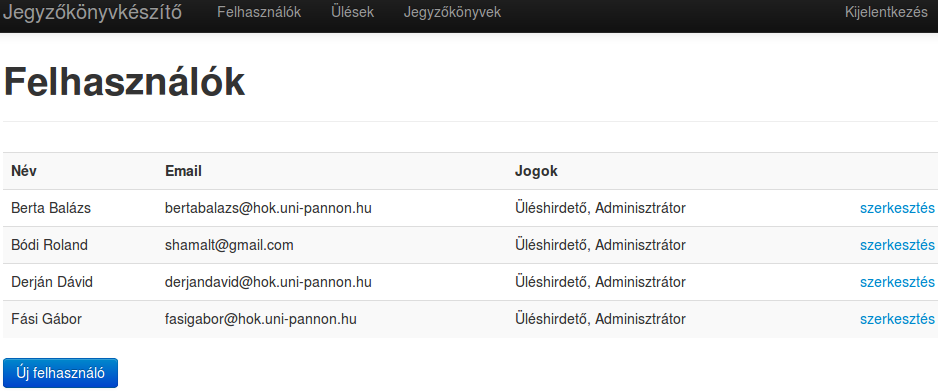
\includegraphics[width=\textwidth]{felhasznalo_lista.png}
    \caption{A felhasználók listája}
    \label{fig:felhasznalo_lista}
\end{figure}

\subsubsection*{Felhasználók szerkesztése}

Most már van linkünk, ami a szerkesztőfelületre mutat, és átadjuk benne a felhasználó azonosítóját. Az action függvényünkben ez alapján lekérjük az adatbázisból és megjelenítjük ez űrlapon.

A lekérést megtehetnénk a függvényünk részeként is, de van rá jobb megoldás: egy saját {\tt ParamConverter} írása. Ezek arra jók, hogy az url-ben kapott értékek alapján a függvényünk rögtön egy {\tt Felhasznalo} példányt kaphat. Korábban, amikor a Dependency Injection Containerről írtam, mutattam azt a kódrészletet, amely a felhasználókat id-ből {\tt Felhasznalo} objektummá átalakító {\tt ParamConverter}t regisztrálja.

Ezek az osztályok egy adott interfészt kell megvalósítsanak, amely két függvényt ír le: az első paraméterként egy osztálynevet kap, és vissza kell adnia, támogatja-e az ilyenre átalakítást. A második magát az alakítást végzi paraméterként kapott {\tt Request} alapján. Ebben a példában az url-ben kapott {\tt id} paraméter alapján kérek az adatbázisból, ha nincs ilyen, hibát dobok, amúgy beállítom a {\tt Request}be a konfigurációban beállitott kulcs alá. Végeredményként az action függvényünk ennyire leegyszerűsödik:

\begin{lstlisting}
public function editAction(Felhasznalo $felhasznalo, Request $request)
{
    $form = $this->createForm(new FelhasznaloType(), $felhasznalo);

    return $this->render("SzakdolgozatFelhasznaloBundle:Felhasznalo:edit.html.twig", array(
        "form"          =>  $form->createView(),
        "felhasznalo"   =>  $felhasznalo,
    ));
}
\end{lstlisting}

Jól látható, hogy már egy felhasználót kapunk bemeneti paraméterként. Létrehozunk egy formot, melyet feltöltünk az ebben található értékekkel, majd a twiggel rendereltetjük a szerkesztés űrlapot tartalmazó template-et. Abban az űrlap egy részlete így néz ki:

\begin{lstlisting}
<form method="post" action="{{ app.request.requesturi }}">
    {{ form_row(form.nev) }}
    {{ form_row(form.email) }}
\end{lstlisting}

Azaz az elküldés POST-tal kell történjen, méghozzá az aktuális url-re. A {\tt form\_row} twig függvények pedig az űrlap egy-egy sorát renderelik, cimkével, mezővel és az esetleges hibaüzenettel. Ennek pontos módját testreszabhatjuk, ahogy én is tettem, hogy a Bootstrapnak megfelelő kimenete legyen.

Az elküldött form feldolgozását ugyanaz a függvény végzi, a formot létrehozó, majd a kimenetet renderelő sor között található ez:

\begin{lstlisting}
if ($request->isMethod("post")) {
    $form->bind($request);

    if ($form->isValid()) {
        $this->getDoctrine()->getManager()->flush();

        return $this->redirect($this->generateUrl("szakdolgozat_felhasznalo_felhasznalo_index"));
    }
}
\end{lstlisting}

Azaz ha az aktuális kérés POST, akkor a kapott értékeket átadjuk a formnak, ekkor megtörténik azok ellenőrzése. Ha minden érték helyes, akkor a Doctrine Entity Managerén meghívjuk a {\tt flush} függvényt, ami a kezelt objektumok (mint a felhasználónk) módosításait menti az adatbázisba. Végül átirányítjuk a felhasználót a listára.

A form példányunk a Symfony2 Form komponensére épít \textendash{} itt egy osztályban leírjuk, milyen mezőket szeretnénk és milyen validálási szabályokkal, a controllerünk pedig a fent látható mértékben leegyszerűsödik. A leírást a {\tt buildForm} függvény végzi, egy részlete:

\begin{lstlisting}
public function buildForm(FormBuilderInterface $builder, array $options)
{
    $builder->add("email", "email", array(
        "label"         =>  "E-mail cím",
        "constraints"   =>  array(
            new Assert\NotBlank(),
            new Assert\Email(),
        ),
    ));

    $builder->add("jogok", "entity", array(
        "class"         =>  "SzakdolgozatFelhasznaloBundle:Jog",
        "expanded"      =>  true,
        "multiple"      =>  true,
    ));

}
\end{lstlisting}

Ebben a példában két mezőt mutatok, az első a felhasználó email címe, amelyhez egy email típusú mező szükséges, valamint kötelező, és szintaktikailag érvényes email cím kell legyen. A második egy adatbázis-entity hivatkozás, méghozzá a Jogra. A fenti beállításokkal egy jelölőnégyzetes listát kapunk, mellyel szabadon meghatározhatjuk, mely jogokkal rendelkezzen a felhasználó. Az űrlap a \ref{fig:felhasznalo_szerkesztes}. ábrán látható.

\begin{figure}[h]
    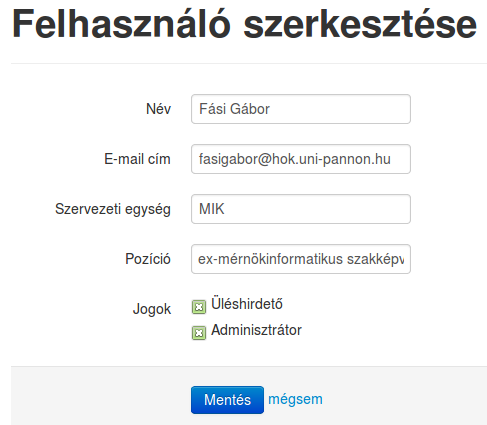
\includegraphics[width=\textwidth]{felhasznalo_szerkesztes.png}
    \caption{A felhasználók szerkesztésére szolgáló űrlap}
    \label{fig:felhasznalo_szerkesztes}
\end{figure}

\subsection{Ülésszervező modul}

A fejlesztés logikusan következő lépése az ülések szervezésére szolgáló modul elkészítése volt. Ez már épít a felhasználókra, úgy mint az ülés hirdetője és meghívottjai. Feladata, hogy a létrehozott üléseket tárolja, az azokhoz feltöltött dokumentumokat kezelje és elérhetővé tegye az elérésükre jogosultaknak. Végül értesítenie kell a meghívottakat arról, hogy ülésük lesz.

\subsubsection*{Adatbázisa}

Ebben a modulban két entitást kell leírnunk, az egyik az ülés, a másik a dokumentum.

A dokumentumot az azonosítójából generált néven tároljuk a szerveren, egy olyan helyen, ami nem közvetlenül elérhető kívülről, így biztosítani tudjuk, hogy csak a hozzáféréssel rendelkező felhasználók tölthetnek le egy-egy csatolmányt. A generált név miatt azonban tárolnunk kell az file eredeti nevét, hogy letöltéskor így tudjuk kiszolgálni.

Az ülésekről tárolunk néhány alapadatot, ezeken kívül több relációval is rendelkezik: tartozhat hozzá akármennyi dokumentum (természetesen akár nulla is), szintén tetszőleges számú meghívott, valamint pontosan egy hirdető. A meghívottak és a hirdető a felhasználó modulban definiált {\tt Felhasznalo} entitásra hivatkozik.

Az adatbázis szerkezete látható a \ref{fig:ules_db}. ábrán. Az {\tt UlesMeghivott} tábla csak az adatbázisban létezik az ülés-meghívott több-több kapcsolat segédtálájaként, entitás nincs hozzá.

\begin{figure}[h]
    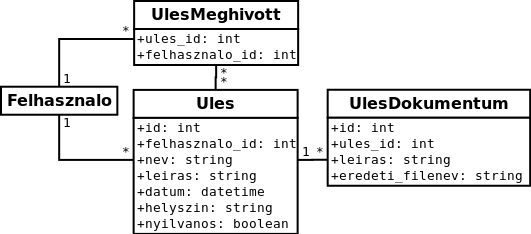
\includegraphics[width=\textwidth]{ules_db.png}
    \caption{Az ülés modul adatbázisának szerkezete}
    \label{fig:ules_db}
\end{figure}

Korábban nem mutattam még példát egy-több kapcsolatra, mint ami az ülés és a dokumentumok közt van. Az {\tt Ules} osztályban az annotáció a következő:

\begin{lstlisting}
/**
 * @ORM\OneToMany(targetEntity="Dokumentum", mappedBy="ules")
 */
protected $dokumentumok;
\end{lstlisting}

A {\tt Dokumentum} osztályban pedig:

\begin{lstlisting}
/**
 * @ORM\ManyToOne(targetEntity="Ules", inversedBy="dokumentumok")
 * @ORM\JoinColumn(name="ules_id", referencedColumnName="id", nullable=false)
 */
protected $ules;
\end{lstlisting}

\subsubsection*{Használati esetek}

Ennek a modulnak a felelőssége az ülések létrehozása, szerkesztése, törlése; azok meghívottjainak és dokumentumainak számontartása; a dokumentumok kiszolgálása jogosultság esetén. Ezek a használati esetek láthatóak a \ref{fig:ules_usecase}. ábrán.

\begin{figure}[h]
    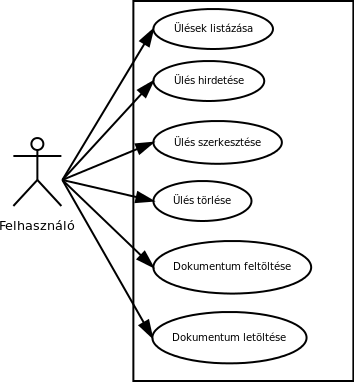
\includegraphics[width=\textwidth]{ules_usecase.png}
    \caption{Az ülésszervező modul használati esetei}
    \label{fig:ules_usecase}
\end{figure}

\subsubsection*{Új ülés hirdetése}

Az üléshirdető joggal rendelkező felhasználók létrehozhatnak új üléseket, megadhatják meghívottjaikat, illetve létrehozás után tölthetnek fel hozzá dokumentumokat. Az üléslista alján található {\it Új ülés} gomb a korábban már látott {\tt is\_granted} függvénnyel van biztosítva, a controllerünk viszont egy eddig nem látott módszerrel: a megfelelő függvény kapott egy annotációt:

\begin{lstlisting}
/**
 * @Secure(roles="ROLE_ULESHIRDETO")
 */
public function newAction(Request $request)
\end{lstlisting}

Ezután a Security komponens az ide mutató összes url elérésekor ellenőrzi, a bejelentkezett felhasználó rendelkezik-e ezzel a joggal, ha nem, automatikusan hibaoldalra irányítja.

Az űrlap a korábban már mutatott adatbázis-séma alapadatait tartalmazza, valamint egy listát a rendszer felhasználóiról, mindegyikhez tartozik egy jelölőnégyzet, amivel azt tudjuk megadni: meghívott-e az illető. Ez látható a \ref{fig:ules_uj}. ábrán. Nagy felhasználószámnál a jelölőnégyzetes megoldás problémás, erre a továbbfejlesztés során szeretnék valami jól használható megoldást találni.

\begin{figure}[h]
    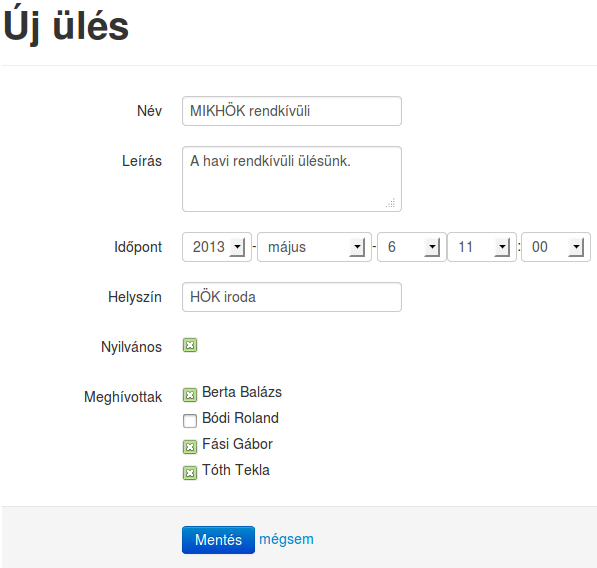
\includegraphics[width=\textwidth]{ules_uj.png}
    \caption{Az új ülés hirdetésére szolgáló űrlap}
    \label{fig:ules_uj}
\end{figure}

\subsubsection*{Dokumentumok kezelése}

Miután kihirdette az ülést, a szerkesztésére szolgáló oldalon a felhasználó tud hozzá tetszőleges számú dokumentumot feltölteni \textendash{} ez akkor hasznos, amikor például az ülés egy belső szabályzat tervezett módosításáról szól, ahogy nem sokkal ezelőtt a Hallgatói Önkormányzat tárgyalta a tervezett TVSz-változtatásokat. A dokumentumoknak egy kötelező mezője van, a leírásuk, ide 255 karakter hosszan bármit lehet írni. Tárolom ezen kívül az eredeti fájlnevet, hogy letöltéskor ugyanazon a néven lehessen menteni.

Ezeket a dokumenentumokat később nyilvános ülés esetén bárki, zárt ülés esetén pedig a meghívottak tudják letölteni. A fájlok olyan helyen vannak tárolva, ami nem elérhető kívülről, így a letöltést mindenképp a rendszeren keresztül kell végezni, ahol van lehetőség a jogosultság ellenőrzésére.

A fájlokat kiszolgáló controller egy {\tt ParamConverter} segítségével rögtön egy {\tt Dokumentum} objektumot kap, lérehoz egy választ, beállítja a letöltéshez szükséges fejléceket és a tartalmat, majd visszatér azzal:

\begin{lstlisting}
public function downloadAction(Dokumentum $dokumentum)
{
    $response = new Response();
    $response->setContent(file_get_contents($dokumentum->getFilename()));
    $response->headers->set("Content-Type", "application/octet-stream");
    $response->headers->set("Content-Disposition", "attachment; filename=" . $dokumentum->getEredetiFilenev());

    return $response;
}
\end{lstlisting}

Az ülés dokumentumainak kezelérésre szolgáló felület látható a \ref{fig:ules_dokumentumok}. ábrán.

\begin{figure}[h]
    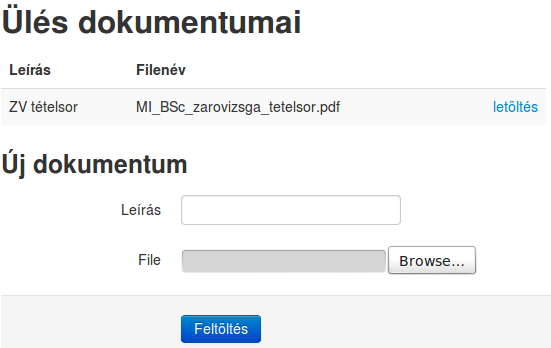
\includegraphics[width=\textwidth]{ules_dokumentumok.png}
    \caption{Az ülés dokumentumainak kezelésére szolgáló felület}
    \label{fig:ules_dokumentumok}
\end{figure}

\subsubsection*{Google Naptár}

A hirdetett ülésekről a rendszer a Google Naptárában létrehoz egy eseményt a rendszerben megadott adatokkal, meghívottakkal. Ennek három fontos előnye van:

\begin{enumerate}
    \item Esemény létrehozásakor a meghívottak emailben értesítőt kapnak, amiben szerepel az ülés címe, leírása, helye és ideje
    \item Esemény módosításakor a meghívottak erről is értesítést kapnak
    \item Az esemény a meghívottak naptárában is látszik, ezzel segítve a teendőik átlátását
\end{enumerate}

A kommunikációt a Google hivatalos klienskönyvtárának segítségével valósítottam meg.

A Symfony2 része egy eseménykezelő komponens. Ebben tetszőleges eseményeket hozhatunk létre, és iratkozhatunk fel rájuk. Erre az egyik lehetőség egy {\it Event Subscriber} osztály készítése, majd regisztrációja:

\begin{lstlisting}
szakdolgozat.ules.gcal_event_subscriber:
    class: Szakdolgozat\UlesBundle\EventSubscriber\GcalEventSubscriber
    arguments: [@session, @doctrine.orm.default_entity_manager]
    tags:
        - { name: "kernel.event_subscriber" }
\end{lstlisting}

Egy statikus függvény visszatérési értékével kell meghatároznunk, mely eseményekre akarunk feliratkozni, és azok mely függvényeket hívják meg:

\begin{lstlisting}
public static function getSubscribedEvents()
{
    return array(
        "ules.new"      =>  "ulesNew",
        "ules.edit"     =>  "ulesEdit",
        "ules.delete"   =>  "ulesDelete",
    );
}
\end{lstlisting}

Definiáltam továbbá egy {\tt GcalEvent} osztályt, az események adataként ilyet továbbítok. Új ülés létrehozásakor a controllerben szükséges kód a következő:

\begin{lstlisting}
$this->get("event_dispatcher")->dispatch("ules.new", new GcalEvent($ules));
\end{lstlisting}

Az {\tt ulesNew} függvényünk gondoskodik a naptárbejegyzés létrehozásáról, valamint annak visszakapott azonosítójának adatbázisba mentéséről \textendash{} erre később az ülés szerkesztésekor és törlésekor lesz szükségünk:

\begin{lstlisting}
public function ulesNew(GcalEvent $event)
{
    $ules = $event->getUles();

    $event = new \Google_Event();
    $this->ulesAdatokEventbe($ules, $event);

    $service = $this->getGoogleCalendarService();
    $created_event = $service->events->insert($this->calendar_id, $event, array("sendNotifications" => true));

    $ules->setGcalEventId($created_event->getId());
    $this->entity_manager->flush($ules);
}
\end{lstlisting}

Azaz egy segédfüggvény használatával az ülés adatait átmásolom egy újonnan létrehozott {\tt Google\_Event} objektumba, majd egy megfelelően konfigurált {\tt Google\_CalendarService} példánynak átadva hozom létre a szerveren az naptárbejegyzést. Végül a létrehozott bejegyzés azonosítóját mentem az ülés adatai közé.

\subsection{Jegyzőkönykészítő modul}

\subsubsection*{Adatbázisának szerkezete}

Ennek a modulnak a feladata tárolni a jegyzőkönyveket, alapadataikkal és elemeikkel, illetve azok sorrendjével együtt. A szerkezete látható a \ref{fig:jegyzokonyv_db}. ábrán, amelyről helytakarékossági okból lehagytam a {\tt Felhasznalo} és az {\tt Ules} táblákat.

\begin{figure}[h]
    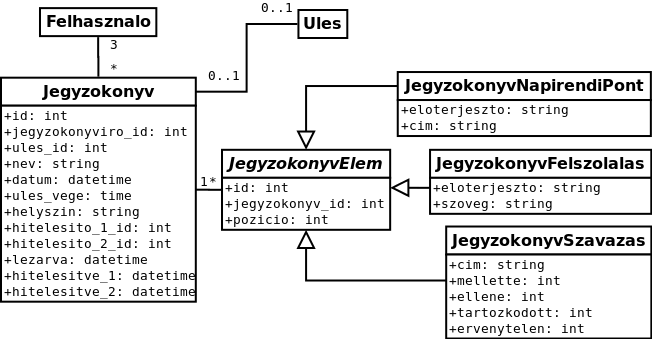
\includegraphics[width=\textwidth]{jegyzokonyv_db.png}
    \caption{A jegyzőkönyvkészítő modul adatbázisának szerkezete}
    \label{fig:jegyzokonyv_db}
\end{figure}

A {\tt Jegyzokonyv} tábla két nem ábrázolt relációval rendelkezik: az egyik a {\tt Felhasznalo} táblára mutat és három mezőre vonatkozik: a jegyzőkönyv írójára és a két hitelesítőre; a másik az {\tt Ules} táblára mutat, és azt jelzi, tartozik-e hozzá ülés. A lezárási, hitelesítési folyamatot dátum mezőkkel ábrázoltam, mert így egyszerre követhető az is, mikor történtek az egyes lépések.

A {\tt JegyzokonyElem} egy absztrakt osztály, a három típusú elem közös mezőit tartalmazza. A Doctrine Single Table Inheritance-ét használom, ezzel az elemet egy közös táblában tárolódnak, plusz egy mezővel, mely megmondja, az adott rekord melyik típusba tartozik. A másik hasonló lehetőség az, amikor elemenként külön táblákban tárolódnak, de mivel az elemek részben közös mezőkkel rendelkeznek, valamint az összes mezőjük kisméretű, a közös táblás tárolás mellett döntöttem. Bár a tárolás így nem optimális, a lekérdezések sebessége ellensúlyozza ezt.

\subsubsection*{Használati esetek}

E modul feladatai közé tartozik az új jegyzőkönyv létrehozása, ami utána csak a készítője (vagy valamely adminisztrátor) által szerkeszthető. A folyamatban levő vagy kész jegyzőkönyveket bárki megtekintheti, ha a hozzájuk tartozó ülés nyilvános, vagy nincs üléshez párosítva; zárt ülés esetén csak annak meghívottjai. Szintén e modul felügyeli a jegyzőkönyvek lezárási folyamatát, valamint képes azokat PDF formátumban exportálni. Ezeken felül az adminisztrátorok tudják a már létező jegyzőkönyvek készítőjét módosítani. Ezen használati esetek láthatóak a \ref{fig:jegyzokonyv_usecase}. ábrán.

\begin{figure}[h]
    \centering
        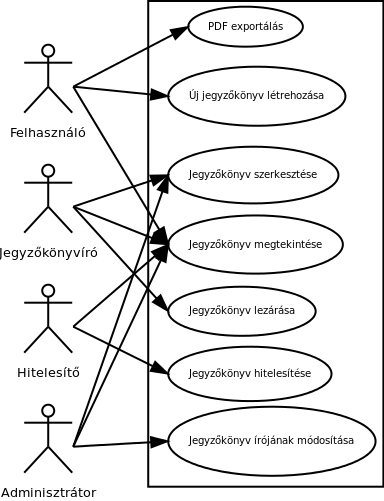
\includegraphics[width=.8\textwidth]{jegyzokonyv_usecase.png}
        \caption{A jegyzőkönyv modul használati esetei}
        \label{fig:jegyzokonyv_usecase}
\end{figure}

\subsubsection*{Új jegyzőkönyv létrehozása}

A jegyzőkönyvek menüpont mindenki által látható, és a felhasználó által látható jegyzőkönyvek listájára mutat. A táblázat alján található gomb az egyik lehetőség az új jegyzőkönyv létrehozására \textendash{} ekkor az nem kapcsolódik üléshez.

A másik lehetőség a felhasználó kezdőlapján található {\it Üléseim} táblázat, amibe pontosan akkor kerül a {\it Jegyzőkönyv létrehozása} link, ha ahhoz az üléshez még nem kapcsolódik jegyzőkönyv.

Mindkét út ugyanarra az űrlapra vezet, ahol először az ülés alapadatait kell megadni. Ha üléshez kapcsolódó jegyzőkönyv készül, akkor ezeket a rendszer automatikusan kitölti, a jegyzőkönyvírónak csak azzal kell foglalkoznia, amit nem tudott, mint például az ülés zárásának időpontja, vagy a jelen levő szavazati jogú tagok száma. Az adatokkal kitöltött űrlap látható a \ref{fig:jegyzokonyv_uj}. ábrán.

\begin{figure}[h]
    \centering
    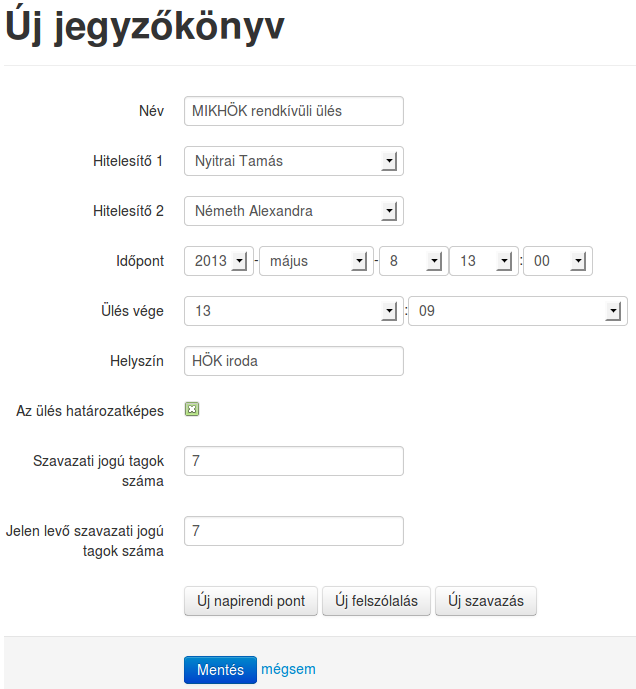
\includegraphics[width=\textwidth]{jegyzokonyv_uj.png}
    \caption{Az új jegyzőköny létrehozására szolgáló űrlap}
    \label{fig:jegyzokonyv_uj}
\end{figure}

Az alapadatok megadása már elég, hogy a jegyzőkönyvet menteni lehessen.

Új jegyzőkönyv-elemeket az űrlap alján található, az egyes típusoknak megfelelő gombokkal lehet; ekkor az új elem a sorrend végére kerül, de a felhasználó egyszerű drag'n'drop módszerrel tetszőleges helyre mozgathatja (ugyanezzel a megoldással átrendezhetőek az elemek a későbbiek során is).

Az egyes elemek vizuálisan jól elkülöníthetőek, ez látható a \ref{fig:jegyzokonyv_szerkesztes}. ábrán. A jobb felső sarkukban található gombbal lehet őket törölni.

\begin{figure}[h]
    \centering
    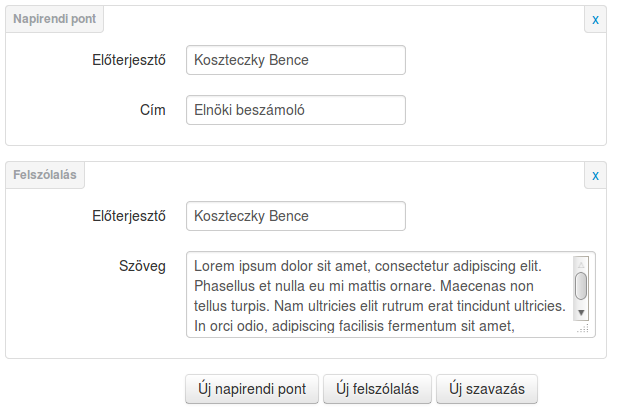
\includegraphics[width=\textwidth]{jegyzokonyv_szerkesztes.png}
    \caption{Jegyzőkönyvelemek}
    \label{fig:jegyzokonyv_szerkesztes}
\end{figure}

\subsubsection*{Szerkesztett jegyzőkönyv mentése}

Az egész rendszernek a legösszetettebb algoritmusa, ennek a működését szeretném bemutatni. Két adatforrást kell összefésülnie: az adatbázisban levőt, valamint a felhasználótól kapottat.

Amikor a szerkesztés űrlapot elküldi a felhasználó, három tömböt kapok: az első a jegyzőkönyv alapadatait tartamazza, a második a jegyzőkönyv elemeit, a harmadik pedig a törölt, korábban már adatbázisba mentett elemek azonosítóit. Az elemeket tartalmazó tömb újabb tömböket tartalmaz, amelyekben találhatóak az egyes elemek adatai.

Szerveroldalon a jegyzőkönyvnek, illetve az elemtípusoknak létrehoztam egy-egy űrlapot a Symfony2 Form komponensében, az azoknak megfelelő mezőkkel illetve validálási szabályokkal. A feldolgozás első lépése az, hogy az adatbázisban található adatokkal és elemekkel létrehozok egy form objektumot a jegyzőkönyvnek és egy-egy darabot az elemeinek.

A következő lépés a létrehozott objektumokhoz az oda tartozó, felhasználótól kapott értékek hozzárendelése. Ennek során figyelem, van-e olyan elem, amelyik érvénytelen értékeket tartalmaz.

Ezután ha az űrlap alapadatai helyesek, és az összes elemet tartalmazó form is helyes, kezdem a kapott adatok adatbázisba tárolását. A jegyzőkönyv már mentve van, itt csak frissíteni kell annak értékeit. Az elemek tömb kulcsának jelentése van:

\begin{itemize}
    \item ha pozitív, akkor már tárolt elemről van szó, a kulcs az azonosítója, és az adatbázisban módosítanunk kell
    \item ha negatív, akkor új elemről van szó, és az adatbázisba beillesztenünk kell
\end{itemize}

A feldolgozást e jelentéseknek megfelelően végzem. A folyamat során figyelek arra is, hogy az elemek sorrendjét helyesen mentsem mind új, mint módosított elemeknél.

A feldolgozás utolsó lépése a törölt elemek adatbázisból eltávolítása. Kliensoldalról egy tömbben megkaptam azok azonosítóit, egyszerűen végigiterálok ezeken, és törlöm őket.

Sikeres mentés után a felhasználót továbbirányítom a jegyzőkönyvek listájára. Ha a mentés során valahol hibás adattal találkozom, akkor a felhasználó visszakapja a szerkesztés űrlapot az általa megadott adatokkal, jelezve azt, melyik hibás és miért.

Ez az algoritmus közel 200 sor hosszú. A továbbfejlesztés során ezt szeretném szétbontani lépésenként külön függvényekbe, amiket egyenként tudok egységtesztelni, hogy a későbbiek során garantáltan ne kerülhessen beléjük hiba.

\subsubsection*{PDF exportálás}

Számos helyen a mai napig papíralapú iktatást használnak, többek között a Hallgatói Önkormányzat irodájában is. Ezt mindenképpen lehetővé kellett tennie rendszeremnek, így a jegyzőkönyveket lehet pdf formátumban exportálni.

Több php nyelvű könyvtár is elérhető, mely ezt teszi lehetővé; a választásom az mPDF-re esett az alábbi okokból:

\begin{itemize}
    \item ma is aktívan fejlesztik
    \item jó a dokumentációja
    \item HTML bemenetből dolgozik
\end{itemize}

Ebből az utolsó a legfontosabb. Ezzel tudtam azt elérni, hogy a későbbiekben a pdf fájlok tetszés szerint testreszabhatóak legyenek anélkül, hogy a rendszer kódjához hozzá kelljen nyúlni. Csak két érték van beégetve: a papír mérete, valamint hogy álló helyzetű legyen.

Az exportálást végző kódrészletet egy külön osztályba tettem, amelyet szolgáltatásként regisztráltam:

\begin{lstlisting}
szakdolgozat.jegyzokonyv.export.pdf:
    class: Szakdolgozat\JegyzokonyvBundle\Export\Pdf
    arguments: [@templating]
\end{lstlisting}

Látható, hogy paraméterként várja a keretrendszer templating szolgáltatását, a twiget. Ennek segítségével a jegyzőkönyvek készítése során használhatóak az abban található ellenőrzések, vezérlési szerkezetek, így akár azt is lehetővé téve, hogy ha nem adminisztrátor exportál, akkor valamilyen vízjelet kapjanak az oldalak.

Az osztályunkban a függvény mindössze pár soros:

\begin{lstlisting}
public function jegyzokonyv(Jegyzokonyv $jegyzokonv)
{
    $mpdf = $this->alapMPDF();

    $mpdf->WriteHTML($this->templating->render("SzakdolgozatJegyzokonyvBundle:Pdf:jegyzokonyv.html.twig", array("jegyzokonyv"   =>  $jegyzokonv)));

    $mpdf->Output($jegyzokonv->getNev() . ".pdf", "I");
}
\end{lstlisting}

Az első sor egy mPDF objektumot hoz létre, mely az alapbeállításokat tartalmazza: a lap mérete, orientációja, valamint hogy mely fájlokban találhatóak a fej- és láblécek leírásai. A második sor ennek beállítja a HTML tartalmát arra, amit a twig generál, majd a harmadik sor visszaadja azt a felhasználónak.

A fejlesztés során elkészítettem egy olyan kimenetet, amely nagyon hasonló ahhoz, amilyet a Hallgatói Önkormányzat most használt rendszere készít, ennek egy részlete látható a \ref{fig:jegyzokonyv_export}. ábrán.

\begin{figure}[h]
    \centering
    
\includegraphics[width=\textwidth]{jegyzokonyv_export.png}
    \caption{Az exportált jegyzőkönyv egy részlete}
    \label{fig:jegyzokonyv_export}
\end{figure}

\subsection{Általános modul}
\todo[inline]{Kell ez vajon?}

% Olyan dolgok, amelyek több modulhoz nyúlnak, mint pl. a kezdőoldal

\section{Az elkészült munka értékelése}

% ide jöhetnek a felhasználói visszajelzések is

\section{Továbbfejlesztési lehetőségek}

Van néhány olyan feladat, amiket nem tartalmaz a vállalt témám, de a jövőben szeretném megvalósítani.

Az első ilyen a keretrendszer frissítése. A fejlesztést a 2.1-es verzióban kezdtem, és annak során adták ki a 2.2-es verziót számos olyan változtatással, amelyek visszafelé nem kompatibilisek. Ezeket szeretném tanulmányozni, és a programom úgy módosítani, hogy ne okozzanak gondot. Ezen túl május végére várható a 2.3-as verzió, amely az első LTS, azaz hosszútávon támogatott változat lesz \textendash{} ez itt három évet jelent.

A második ilyen újabb authentikációs módok hozzáadása. Jelenleg csak Google fiókkal lehet belépni, de ezen belül nincs korlátozás. Viszonylag kevés munkával meg lehet oldani egyéb, OpenID-kompatibilis szolgáltatókkal való belépést, valamivel több munkával pedig a hagyományos, felhasználónév-jelszó használatával történőt is.

A harmadik ilyen a mobileszközök használhatóságának vizsgálata. Egy mai mobiltelefon kijelzője túl kicsi, hogy hosszabb szöveg bevitelét tegye lehetővé, de a terjedő tabletek már elég nagyok. A megjelenítésre használt Bootstrap keretrendszer ezeket valamennyire támogatja, de rendelkezésemre álló eszköz híján ezt tesztelni nem tudtam.

Az utolsó ilyen a jegyzőkönyvtípusok támogatása. Jelenleg csak egyet támogat a rendszer, de már felmerült az igény, hogy többet is tegyen lehetővé. Ennek hatása csak az exportált PDF kinézetére terjed, a létrehozási, szerkesztési és lezárási folyamat minden esetben ugyanaz lenne.

\renewcommand{\bibname}{Irodalomjegyzék}
\bibliographystyle{pemik}
\bibliography{irodalomjegyzek}

\end{document}
